\documentclass{article}
	\usepackage{graphicx}
	\begin{document}
		\begin{center}\textbf{Bo Zhang\\01063214\\}
		\end{center}
		\noindent
		\textbf{Task 1:}\\
		Demonstrate that you know how to use "curl" well enough to correctly POST data to a form.  Show that the HTML response that is returned is "correct".  That is, the server should take the arguments you POSTed and build a response accordingly.  Save the HTML response to a file and then view that file in a browser and take a screen shot.\\\\
		\textbf{Curl command:} curl -d "firstname=Roy\&lastname=Zhang" http://quiet-waters-1228.herokuapp.com/echo\\\\
		\textbf{HTML response:}\\
			$<$!DOCTYPE html$>$\\
			$<$html$>$\\
			$<$head$>$\\
			\indent
			  $<$title$>$Unix and Linux Commands for Developers$<$/title$>$\\
			\indent
			  $<$link href="/assets/application.css" media="all" rel="stylesheet" /$>$\\
			\indent
			  $<$script src="/assets/application.js"$>$$<$/script$>$\\
			$<$/head$>$\\
			$<$body$>$\\

			  $<$p$>$\\
			\indent\indent
			    $<$strong$>$url:$<$/strong$>$\\
			\indent\indent
			    $<$span$>$\\
			\indent\indent\indent
			      http://quiet-waters-1228.herokuapp.com/echo\\
			\indent\indent
			    $<$/span$>$\\
			\indent
			  $<$/p$>$\\
			\indent
			  $<$p$>$\\
			\indent\indent
			    $<$strong$>$parameters:$<$/strong$>$\\
			\indent\indent
			    $<$span$>$\\
			\indent\indent\indent
			      \{"firstname"=$>$"Roy", "lastname"=$>$"Zhang"\}\\
			\indent\indent
			    $<$/span$>$\\
			\indent
			  $<$/p$>$\\
			\indent
			  $<$p$>$\\
			\indent\indent
			    $<$strong$>$method:$<$/strong$>$\\
			\indent\indent
			    $<$span$>$\\
			\indent\indent\indent
			      POST\\
			\indent\indent
			    $<$/span$>$\\
			\indent
			  $<$/p$>$\\
			\indent
			  $<$p$>$\\
			\indent\indent
			    $<$strong$>$body:$<$/strong$>$\\
			\indent\indent
			    $<$span$>$\\
			\indent\indent\indent
			      firstname=Roy\&lastname=Zhang\\
			\indent\indent
			    $<$/span$>$\\
			\indent
			  $<$/p$>$\\\\
			$<$/body$>$\\
			$<$/html$>$\\\\
		\textbf{Screen shot:}\\
		\fbox{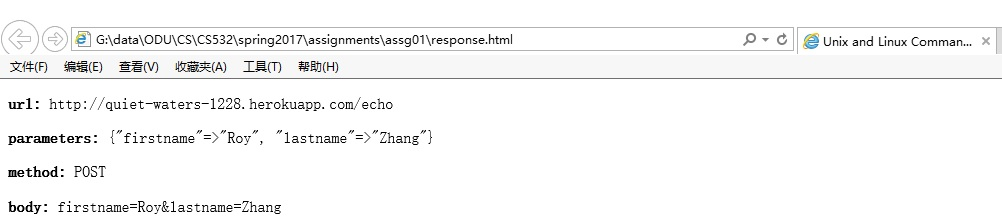
\includegraphics[width=1.2\textwidth]{response.jpg}}\\\\
		\textbf{Note:} I found this website from "http://conqueringthecommandline.com/book/curl"\\\\\\
		\textbf{Task 2:} Write a Python program that:\\
		\indent1. takes as a command line argument a web page\\
		\indent2. extracts all the links from the page\\
		\indent3. lists all the links that result in PDF files, and prints out the bytes for each of the links.  (note: be sure to follow all the redirects until the link terminates with a "200 OK".)\\
		\indent4. show that the program works on 3 different URIs, one of which needs to be:\\
		\indent http://www.cs.odu.edu/~mln/teaching/cs532-s17/test/pdfs.html\\\\
		\textbf{Algorithm:}\\
		\indent1. Ask to input a URI\\
		\indent2. Open this URI and save it into an html object\\
		\indent3. Extracts all the links from the html object\\
		\indent4. Open all the links 1 by 1 and check their Content-Type from the response\\
		\indent5. If the Content-Type is PDF, get the URI from the response of the opened link and print it\\
		\indent6. Print the Content-Length from the response of the opened link\\\\
		\textbf{Results:}\\
		\indent1. http://www.cs.odu.edu/\~{}mln/teaching/cs532-s17/test/pdfs.html\\
		\fbox{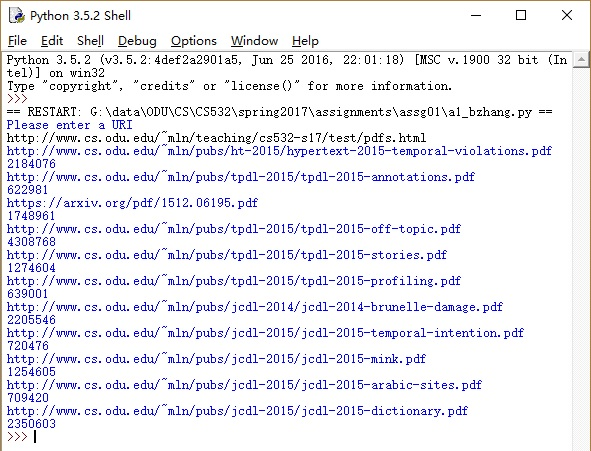
\includegraphics[width=1\textwidth]{result.jpg}}\\\\
		\indent2. http://www.cs.odu.edu/\~{}mln/\\
		\fbox{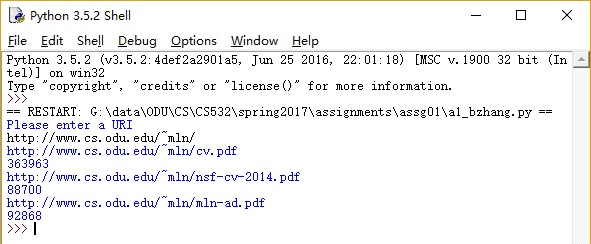
\includegraphics[width=1\textwidth]{result2.jpg}}\\\\
		\indent3. http://www.cs.odu.edu/\~{}mln/teaching/\\
		\fbox{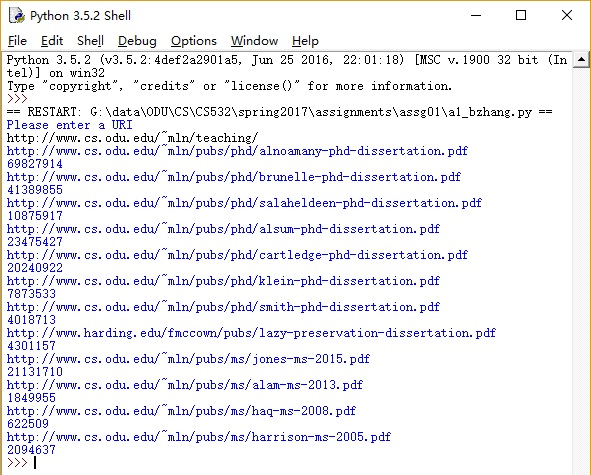
\includegraphics[width=1\textwidth]{result3.jpg}}\\\\\\
		\textbf{Task 3:} Consider the "bow-tie" graph in the Broder et al. paper (fig 9):\\
		http://www9.org/w9cdrom/160/160.html\\\\
		Now consider the following graph:\\\\
		A --$>$ B\\
		B --$>$ C\\
		C --$>$ D\\
		C --$>$ A\\
		C --$>$ G\\
		E --$>$ F\\
		G --$>$ C\\
		G --$>$ H\\
		I --$>$ H\\
		I --$>$ K\\
		L --$>$ D\\
		M --$>$ A\\
		M --$>$ N\\
		N --$>$ D\\
		O --$>$ A\\
		P --$>$ G\\\\
		For the above graph, give the values for:\\\\
		IN: 3 (M, O, P)\\
		SCC: 4 (A, B, C, G)\\
		OUT: 2 (D, H)\\
		Tendrils: 4 (N, L, I, K)\\ 
		Tubes: 1 (M--$>$N--$>$D)\\
		Disconnected: 2 (E, F)\\
	\end{document}